\RequirePackage{luatex85}
\documentclass[amsmath]{article}
\usepackage{amsmath}
\usepackage{amssymb}
\usepackage{geometry,contour}
\usepackage{tikz}
\usetikzlibrary{shapes,snakes}
\usetikzlibrary{shapes.geometric, arrows}
\usetikzlibrary{decorations.text}

\geometry{legalpaper, landscape, margin=0.0in}
\paperheight 2.1in
\paperwidth 3.1in


\begin{document}
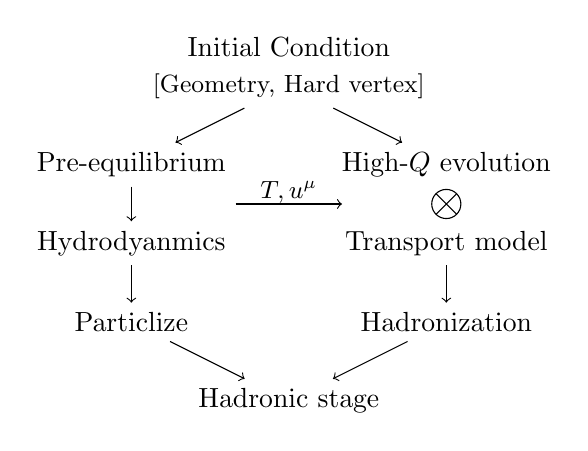
\begin{tikzpicture}[cross/.style={path picture={ 
  \draw[black]
(path picture bounding box.south east) -- (path picture bounding box.north west) (path picture bounding box.south west) -- (path picture bounding box.north east);
}}]

\node (A0) at (4,3) {Initial Condition};
\node (A) at (4,2.5) {\small [Geometry, Hard vertex]};
\node (B) at (2,1.5) {Pre-equilibrium};
\node (C) at (2,.5) {Hydrodyanmics};
\node (D) at (2,-.5) {Particlize};
\node (E) at (4,-1.5) {Hadronic stage};

\node (B2) at (6,1.5) {High-$Q$ evolution};
\node [draw,circle,cross,minimum width=.37 cm] (BC) at (6,1){}; 
\node (C2) at (6,.5) {Transport model};
\node (D2) at (6, -.5) {Hadronization};

\draw[->] (A) edge (B);
\draw[->] (B) edge (C);
\draw[->] (C) edge (D);
\draw[->] (D) edge (E);

\node (a) at  (3.2, 1) {};
\node (b) at  (4.8, 1) {};
\draw[->] (a) edge (b); 
\node (c) at  (4, 1.15) {\small $T, u^\mu$};

\draw[->] (A) edge (B2);
\draw[->] (C2) edge (D2);
\draw[->] (D2) edge (E);
\end{tikzpicture}
\end{document}




